\begin{itemize}
\item Use data-parallel model to scale to many cores, but adopt shared-address space model allowing threads on the same core to communicate
\item A GPU is built around an array of Streaming Multiprocessors (SMs)
\item a GPU with more multiprocessors will automatically execute a multithreaded program in less time than that with fewer multiprocessors
\item CUDA blocks map to GPU cores (streaming multiplrocessors); Warps are groups of (32) threads; 1024 threads per block (cap. 2)
\item total number of warps in a block = ceil$(\frac{T}{W_{\text{size}}},1)$ where $T$ is threads $\#$ per block; $W_{\text{size}} = 32$; rounded to the nearest multiply of 1
\end{itemize}
\begin{minipage}{0.5\linewidth}
  \section*{Kernels}
  \flushleft
  \begin{itemize}
  \item CUDA C++ functions $\to$ \emph{kernels}
  \item executed $N$ times in parallel by $N$ different CUDA threads
  \item defined using \textcolor{Red}{\texttt{\_\_global\_\_}} specifier
  \item \emph{must} return nothing (\texttt{void})
  \item execution configuration \texttt{<<<B,T>>>} specifies two key structures:
    \begin{enumerate}
    \item number of blocks in each dim
    \item threads per block in each dim
    \end{enumerate}
  \item each thread has a unique ID
  \item thread IDs can be up to 3-dim
  \end{itemize}
\end{minipage}
\begin{minipage}{0.5\linewidth}
\begin{lstlisting}[language=C++,xleftmargin=1pt]
// Kernel definition
__global__ void VecAdd(
  float* A, float* B, float* C)
{
  int i = threadIdx.x;
  C[i] = A[i] + B[i];
}

int main()
{
  // invoke kernel with N threads
  VecAdd<<<1, N>>>(A, B, C);
}
\end{lstlisting}
\end{minipage}
\begin{minipage}{0.5\linewidth}
  \section*{Blocks \& thread IDs in 1D,2D,3D}
  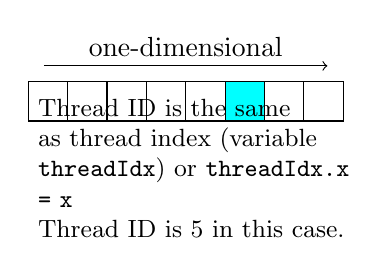
\begin{tikzpicture}
    % 1D block of 8 threads (each as a square)
    \foreach \x in {0,0.5,1,1.5,2,3,3.5}
    {
      \draw (\x,0) rectangle (\x+0.5,0.5);
    }
    % the specific thread square for demo
    \draw[fill=Cyan] (2.5,0) rectangle (3,0.5);

    % Dimension
    \draw[->] (.2,.7) -- (3.8,.7) node[midway,above]{one-dimensional};

    \node[text width=4cm,yshift=-.6cm, ,anchor=west,font=\small]
    {
      Thread ID is the same as thread index (variable \texttt{threadIdx}) or \texttt{threadIdx.x = x}\\
      Thread ID is 5 in this case.
    };
  \end{tikzpicture}
\end{minipage}
\begin{minipage}{0.5\linewidth}
  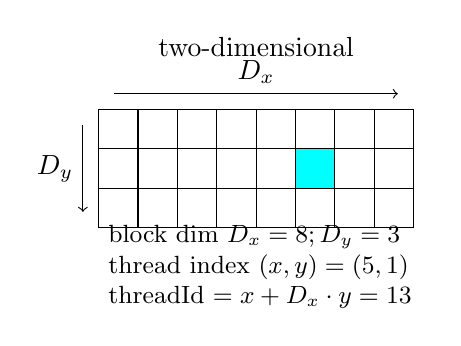
\begin{tikzpicture}
    % 2D block of 24 threads (each as a square)
    \foreach \x in {0,0.5,1,1.5,2,2.5,3,3.5}
    {
      % \draw (\x,1.5) rectangle (\x+0.5,2);
      \draw (\x,1) rectangle (\x+0.5,1.5);
      \draw (\x,0.5) rectangle (\x+0.5,1);
      \draw (\x,0) rectangle (\x+0.5,0.5);
    }
    % the specific thread square for demo
    \draw[fill=Cyan] (2.5,.5) rectangle (3,1);

    % Dimension
    \node (2d) at (2,2.3) {two-dimensional};
    \draw[->] (.2,1.7) -- (3.8,1.7) node[midway,above]{$D_x$};
    \draw[->] (-.2,1.3) -- (-.2,.2) node[midway,left]{$D_y$};

    \node[text width=4cm,yshift=-.5cm,anchor=west,font=\small]
    {
      block dim $D_x = 8; D_y = 3$\\
      thread index $(x, y) = (5,1)$\\
      threadId $= x + D_x \cdot y = 13$
    };
  \end{tikzpicture}
\end{minipage}
\begin{minipage}{0.5\linewidth}
  \begin{center}
    three-dimensional
  \end{center}
  \includegraphics[width=\linewidth]{sec/3dcuda}
\end{minipage}
\begin{minipage}{0.5\linewidth}
  \flushleft
  \begin{itemize}
  \item threadID = $x + y\cdot D_x + z\cdot D_x\cdot D_y$
  \item a thread with index $(x,y,z)$ in 3D-block:
    \begin{itemize}[label=-]
    \item \texttt{threadIdx.x = x}
    \item \texttt{threadIdx.y = y}
    \item \texttt{threadIdx.z = z}
    \end{itemize}
  \item $D_x = \texttt{blockDim.x}$
  \item $D_y = \texttt{blockDim.y}$
  \item $D_z = \texttt{blockDim.z}$
  \end{itemize}
\end{minipage}
\begin{itemize}
\item A thread block of $16\times 16$ (256 threads) is a common choice
\item Thread blocks must execute independently: must be possible to execute in any order, in parallel or in series
\item Threads within a block can cooperate via shared memory (low-latency, like L1 cache) and by synchronizing their execution (\texttt{\_\_syncthreads()})
\end{itemize}
\columnbreak
\begin{tabular}{l|ll}
  \hline
  Var & Type & Contain\\
  \hline
  \texttt{gridDim} & \texttt{dim3} &  the dimensions of the grid (\texttt{gridDim.x,.y,.z})\\
  \texttt{blockIdx} & \texttt{unit3} &  the block index within the grid (\texttt{.x,.y,.z})\\
  \texttt{blockDim} & \texttt{dim3} &  the dimensions of the block (\texttt{blockDim.x,.y,.z})\\
  \texttt{threadIdx} & \texttt{uint3} &  the thread index within the grid (\texttt{.x,.y,.z})\\
  \texttt{warpSize} & \texttt{int} &  warp size in threads\\
  \hline
  \multicolumn{3}{l}{\texttt{dim3} is an integer vector type used to specify dimensions}\\
  \multicolumn{3}{l}{If a var is of\texttt{dim3}, any component left unspecified is inited to 1}\\
  \hline
\end{tabular}
\subsection*{Execution Configuration (EC) \texttt{<<<Dg, Db, Ns, S>>>}}
\begin{minipage}{0.5\linewidth}
  \flushleft
  \begin{itemize}
  \item any call to \texttt{\_\_global\_\_} fn must specify EC for the call
  \item args in \texttt{<<<...>>>} are evaluated before actual function arguments
  \item If any of \texttt{Dg}, \texttt{Db} or \texttt{Ns} greater than the max allowed, fn call fails
  \end{itemize}
\end{minipage}
\begin{minipage}{0.5\linewidth}
\begin{lstlisting}[language=C++,xleftmargin=1pt]
// the declared kernel here
__global__ void Fn(float* param);

// must be called like this
Fn<<< Dg, Db, Ns >>>(param);
// Ns is optional; defaults to 0
\end{lstlisting}
\end{minipage}
\begin{tabular}{p{0.3cm}|p{1.6cm}l}
  \hline
  Arg & Type & Specify\\
  \hline
  \texttt{Dg} & \texttt{dim3} & the dimension and size of the grid$^1$\\
  \texttt{Db} & \texttt{dim3} & the dimension and size of each block$^2$ \\
  \texttt{Ns} & \texttt{size\_t} & the number of bytes in shared memory$^3$ (per block)\\
  \texttt{S} & \texttt{cudaStream\_t} &the associated stream; defaults to 0\\
  \hline
  \multicolumn{3}{l}{1. \texttt{Dg.x * Dg.y * Dg.z} = number of blocks being launched}\\
  \multicolumn{3}{l}{2. \texttt{Db.x * Db.y * Db.z} = number of threads per block}\\
  \multicolumn{3}{l}{3. dynamically allocated for this call; (+ the statically allocated mem) }\\
  \hline
\end{tabular}
\begin{minipage}{0.5\linewidth}
  \begin{itemize}
  \item Executed on the device
  \item  Callable from the host
  \item must have \texttt{void} return type
  \item cannot be a member of a class
  \item returns before the device has completed its execution
  \item Callable from the device (5.0+)
  \end{itemize}
\end{minipage}
\begin{minipage}{0.5\linewidth}
\begin{lstlisting}[language=C++,xleftmargin=1pt]
int main()
{
  // Call  hello( ) kernel
  hello<<< 1, 4 >>>( );// Async!

 // Exec print without any waiting
 printf("CPU: Hello World!\n");
}
\end{lstlisting}
\end{minipage}
% __device__
\begin{minipage}{0.5\linewidth}
  \subsection*{\textcolor{Red}{\texttt{\_\_device\_\_}} execution space specifier}
  \flushleft
  \begin{itemize}
  \item Executed on the device
  \item Callable from the device only
  \item \emph{cannot} be used together with \texttt{\_\_global\_\_}
  \end{itemize}
\end{minipage}
% __host__
\begin{minipage}{0.5\linewidth}
  \subsection*{\textcolor{Red}{\texttt{\_\_host\_\_}} execution space specifier}
  \flushleft
  \begin{itemize}
  \item Executed on the host
  \item Callable from the host only
  \item \emph{cannot} be used together with \texttt{global}
  \end{itemize}
\end{minipage}
% without __host__
\begin{minipage}{0.5\linewidth}
\begin{lstlisting}[language=C++,xleftmargin=1pt,xrightmargin=2pt]
__host__ func() // equivalent to
func()          // without __host__
\end{lstlisting}
\end{minipage}
\begin{minipage}{0.5\linewidth}
\begin{lstlisting}[language=C++,xleftmargin=2pt]
__host__ __device__ func() {};
// compiled for host and device
\end{lstlisting}
\end{minipage}
% Shared
\subsection*{\texttt{\_\_shared\_\_} memory space specifier (optionally used with \texttt{\_\_device\_\_})}
\begin{minipage}{0.5\linewidth}
  \flushleft
  \begin{itemize}
  \item Resides in the shared memory space of a thread block
  \item Has the lifetime of the block
  \item Has a distinct object per block
  \item only accessible from all the threads within the block
  \item Does not have a constant address
  \end{itemize}
\end{minipage}
\begin{minipage}{0.5\linewidth}
\begin{lstlisting}[language=C++,xleftmargin=1pt,framexbottommargin=2pt]
for (m=0; m<SOME; ++m) {
  ...
  // Shared mem to store Asub/Bsub
  __shared__ float As[BLOCK_SIZE];
  __shared__ float Bs[BLOCK_SIZE];
  ...
}
\end{lstlisting}
\end{minipage}
typical programming pattern for shared memeory
\begin{enumerate}
\item Load data from device memory to shared memory
\item Sync with all the other threads of the block so that each thread can safely read shared memory locations populated by different threads
\item Process the data in shared memory
\item Sync again if necessary to make sure shared memory already updated with the results
\item Write the results back to device memory
\end{enumerate}
\columnbreak
\section*{Overall Performance Optimization Strategies (4)}
\subsection*{1.Maximize parallel execution to achieve maximum utilization}
\begin{itemize}
\item Exposes as much parallelism as possible
\item Efficiently maps this parallelism to the various components of the system to keep them busy most of the time
\item App level:
  \begin{enumerate*}
  \item serial workloads to the host
  \item parallel workloads to the devices
  \item use \texttt{\_\_syncthreads()} and shared memory within same kernel call
  \item use asynchronous functions calls and streams
  \end{enumerate*}
\item Devce level:
  \begin{enumerate*}
  \item maximize parallel execution between the multiprocessors of a device
  \item use streams to enable enough kernels to execute concurrently
  \end{enumerate*}
\item MP Level: number of threads per block should be a multiple of the warp size to avoid wasting computing resources with under-populated warps as much as possible
\end{itemize}
\subsection*{2.Optimize memory usage to achieve maximum memory throughput}
\begin{itemize}
\item minimize data transfers between the host and the device (move more code onto device despite of less parallelism)
\item batch many small transfers into a single large transfer
\item on systems with front-side bus, use page-locked host memory
\item if with mapped page-locked memory, no need to allocate any device mem as data transfers are implicitly performed
\item minimize data transfers between global memory and device by maximizing use of on-chip memory: shared memory and caches
\item maximize coalescing (global mem):
  \begin{enumerate*}
  \item follow the most optimal access patterns based on 5.x+ compute capability
  \item use data types that meet the size and alignment requirement
  \item pad data in some cases, when accessing a two-dimensional array
  \end{enumerate*}
\end{itemize}
\subsection*{3.Optimize instruction usage to achieve max instruction throughput}
\begin{itemize}
\item Minimize the use of arithmetic instructions with low throughput; this includes trading precision for speed when it does not affect the end result, such as using intrinsic instead of regular functions, single-precision instead of double-precision, or flushing denormalized numbers to zero;
\item Minimize divergent warps caused by control flow instructions
\item Reduce the number of instructions by optimizing out sync points whenever possible or using restricted pointers (\texttt{\_\_restrict\_\_})
\item for control flow that depends on the thread ID, the ctrl cond should minimize the number of divergent warps (\texttt{threadIdx / warpSize}).
\end{itemize}
\subsection*{4.Minimize memory thrashing}
\begin{itemize}
\item Try to size your allocation to the problem at hand. Don’t try to allocate all available memory with \texttt{cudaMalloc}/\texttt{cudaMallocHost}/\texttt{cuMemCreate}, as this forces memory to be resident immediately and prevents other applications from being able to use that memory $\to$ more pressure on operating system schedulers or just prevent other applications using the same GPU from running entirely
\item Try to allocate memory in appropriately sized allocations early in the application and allocations only when the application does not have any use for it.  Reduce the number of \texttt{cudaMalloc}+\texttt{cudaFree} calls in the application, especially in performance-critical regions
\item If an application cannot allocate enough device memory, consider falling back on other memory types such as \texttt{cudaMallocHost} or \texttt{cudaMallocManaged}, which may not be as performant, but will enable the application to make progress.
\item For platforms that support the feature, \texttt{cudaMallocManaged} allows for oversubscription, and with the correct \texttt{cudaMemAdvise} policies enabled, will allow the application to retain most if not all the performance of \texttt{cudaMalloc}. \texttt{cudaMallocManaged} also won’t force an allocation to be resident until it is needed or prefetched, reducing the overall pressure on the operating system schedulers and better enabling multi-tenet use cases.
\end{itemize}
